\chapter{Data}
\label{chap:data}

This chapter discusses the datasets used in the thesis, as well as the pre and post-processing steps that are performed in order to facilitate the training and validation of the proposed method. In addition to this, a couple of concepts that motivate the choices or that are directly used in the process of the data are explained with the help of illustrations. 

The main dataset used in the thesis is \textit{Human3.6M}: Large Scale Datasets and Predictive Methods for 3D Human Sensing in Natural Environments \cite{H3.6}. Most of the related works benchmark their methods on Human3.6M and it also is freely accessible to academics on request. For further evaluation of model performance in the wild, outdoor datasets that do not have 3D ground truth such as \textit{3DPW}: 3D Poses in the Wild \cite{3dpw} would be used.

\begin{figure}[h]
    \centering
    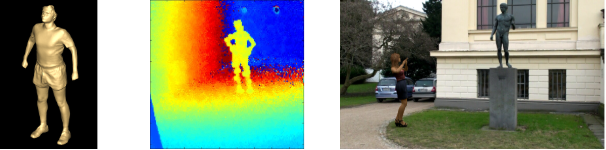
\includegraphics[width=\textwidth]{figures/h36/modlities.png}
    \caption{Additional modalities such as (from left to right) Full body model, depth from time of flight and mixed reality data are availble in Human3.6M dataset \cite{H3.6}. These datasets can be used for human body estimation, depth map estiamtion or inferring absolute 2D or 3D pose directly from full image i.e without cropping the region with a single person.}
    \label{fig:h36_modality}
\end{figure}

\section{Human3.6M}
Human3.6M is a large scale indoor dataset with 3.6 million human poses collected with 4 cameras at different angles using a highly accurate maker-based \ac{mocap} system. The dataset constitutes 15 diverse motion and actions in various everyday scenarios namely, Directions, Discussion, Eating, Greeting, Phoning, Photo, Posing, Purchases, Sitting, Sitting Down, Smoking, Waiting, WalkDog, Walking, and WalkTogether. These actions are performed by 11 professional actors wearing a variety of realistic clothing. The datasets provides synchronized 2D and 3D data including full-body scans as shown in Fig \ref{fig:h36_modality}. It also includes mixed-reality test data created using animated human models to cover huge variations of background, clothing, illumination, occlusion, and camera angles.

The data of interest is mainly the 2D pose for training, 3D poses for evaluation and images for qualitative analysis as it is sometimes challenging even for the human eye to estimate 3D pose just from the 2D skeleton. Both the poses are composed of 17 joints or keypoint annotations namely, Pelvis (also referred to as Root), Torso, Neck, Nose, Head, right and left - Hip, Knee, Ankle, Shoulder, Elbow, Wrist. An image sample from the dataset with its corresponding 2D and 3D pose is illustrated in the Fig \ref{fig:h36_sample}. 

\begin{figure}
    \centering
    \begin{subfigure}[b]{0.3\textwidth}
        \centering
        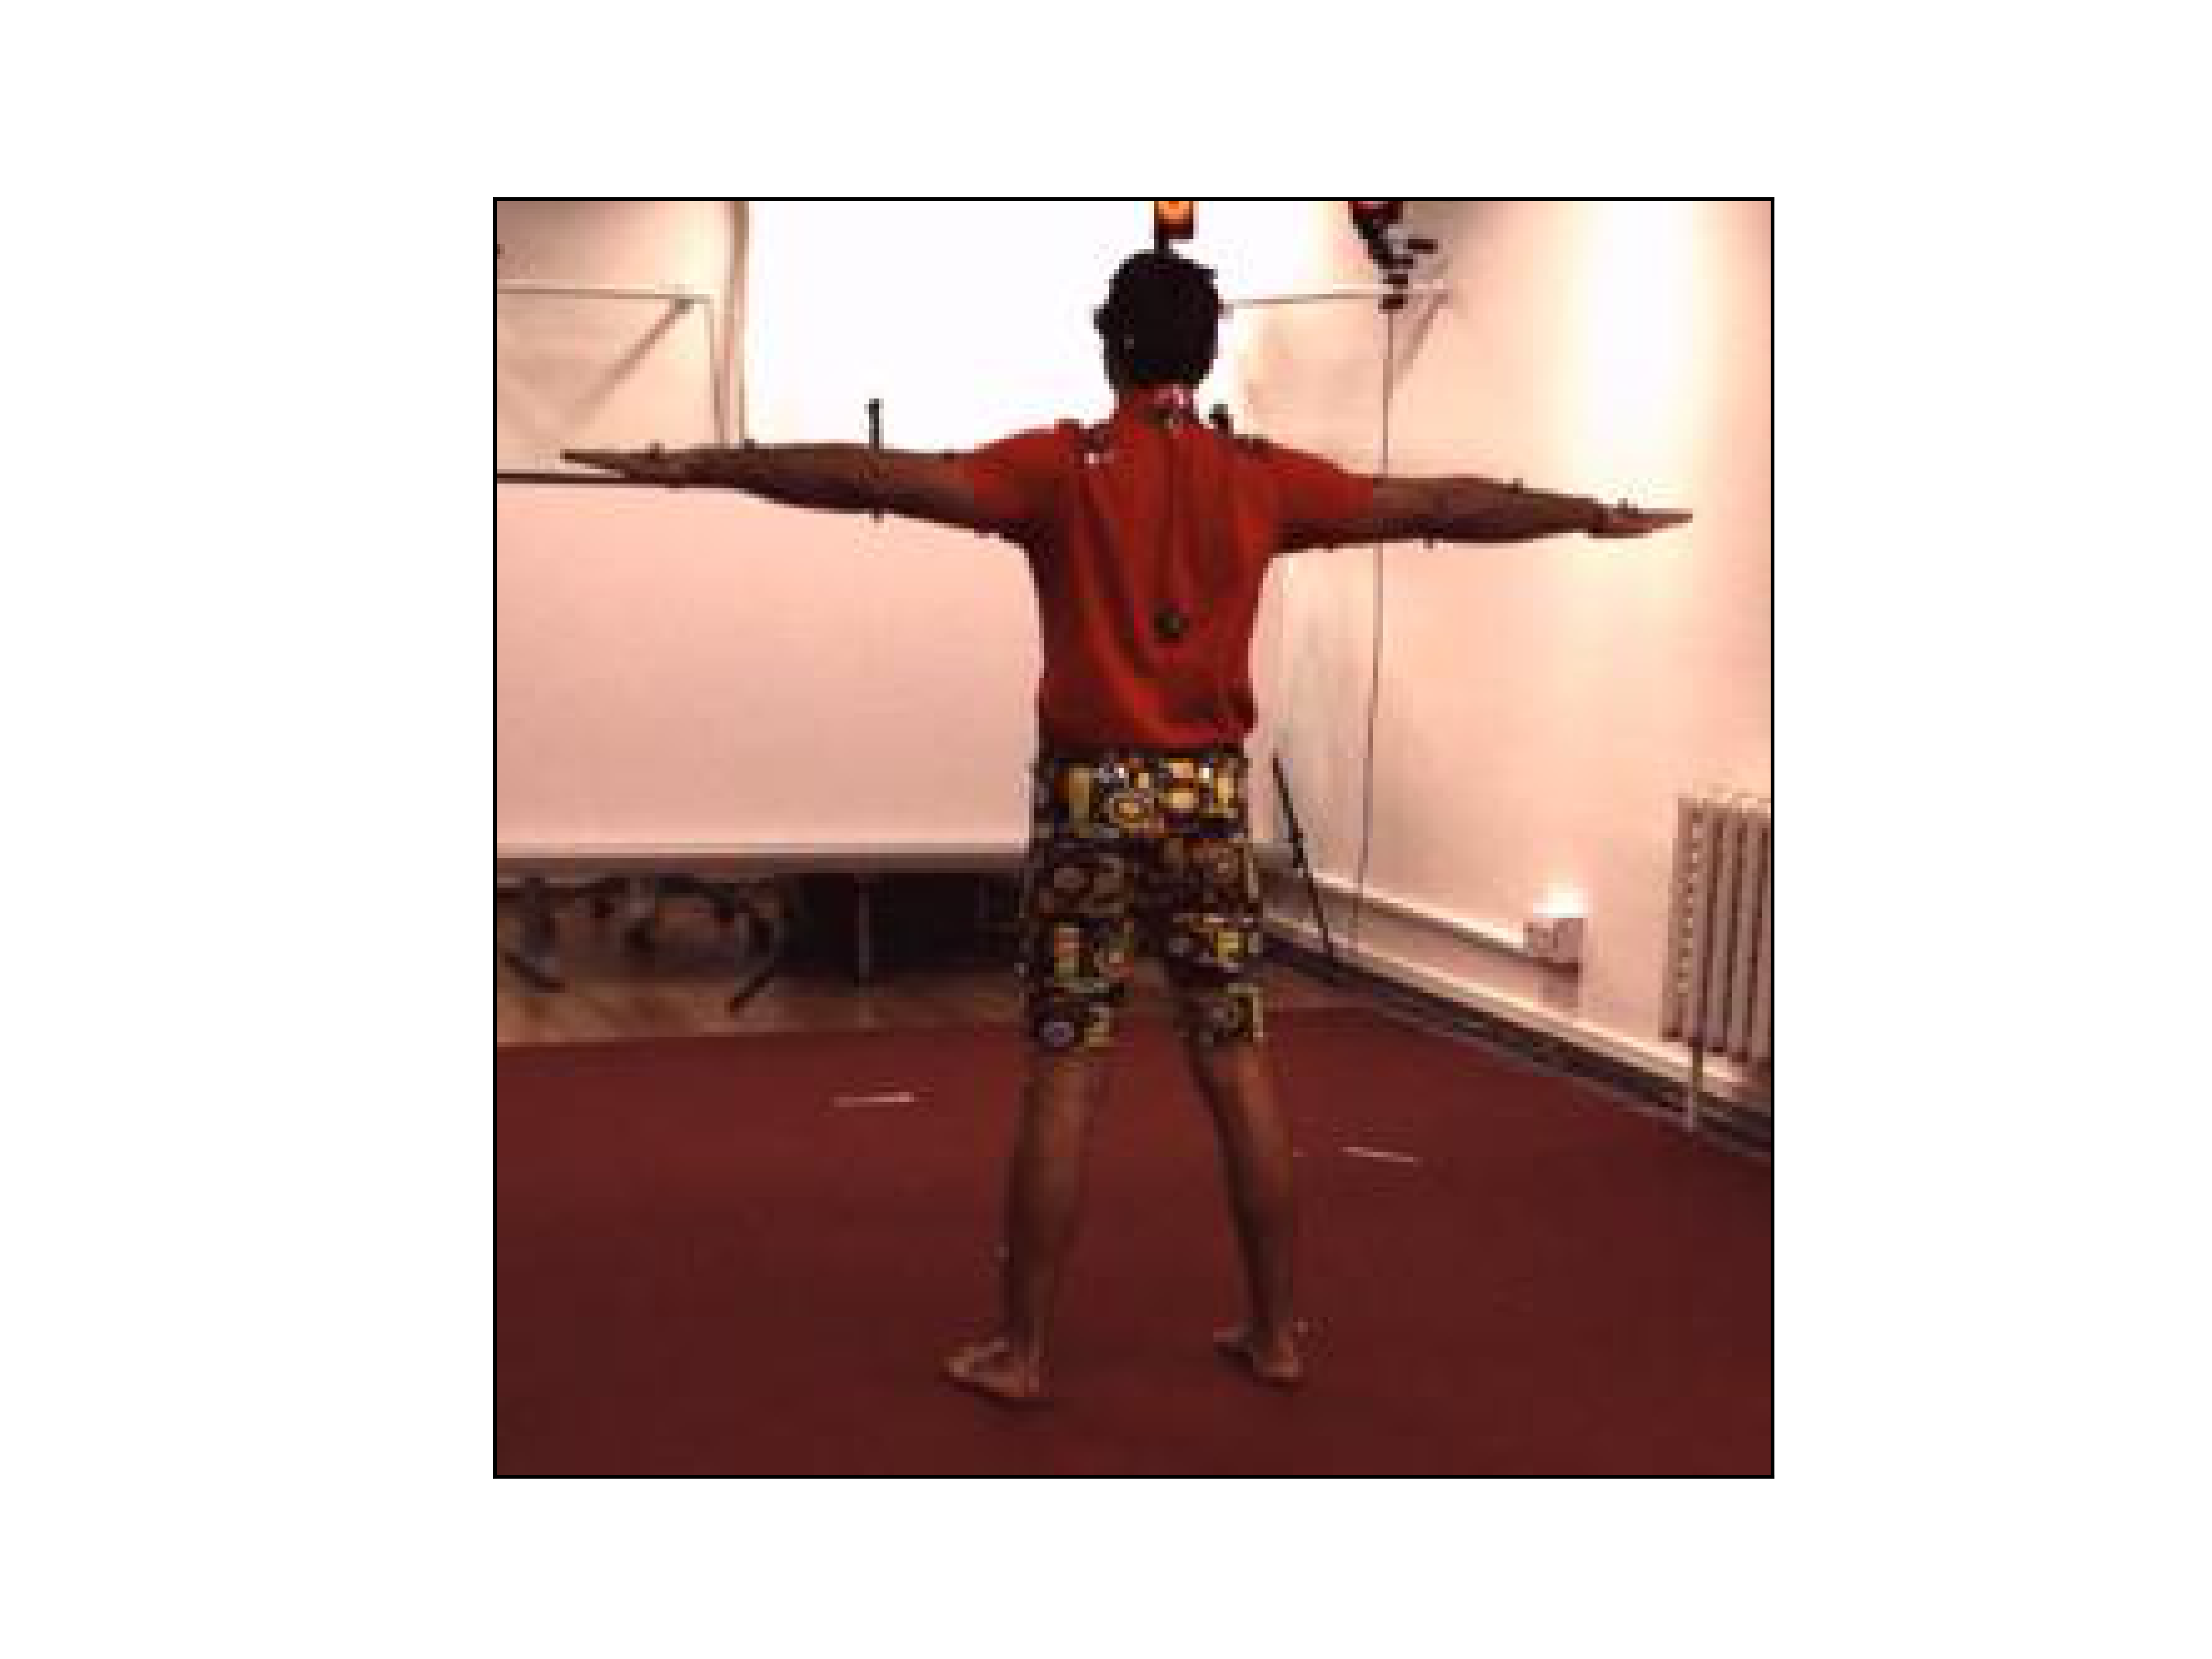
\includegraphics[width=\textwidth]{figures/h36_viz/h36image.png}
        \caption{}
    \end{subfigure}
    \hfill
    \begin{subfigure}[b]{0.3\textwidth}
        \centering
        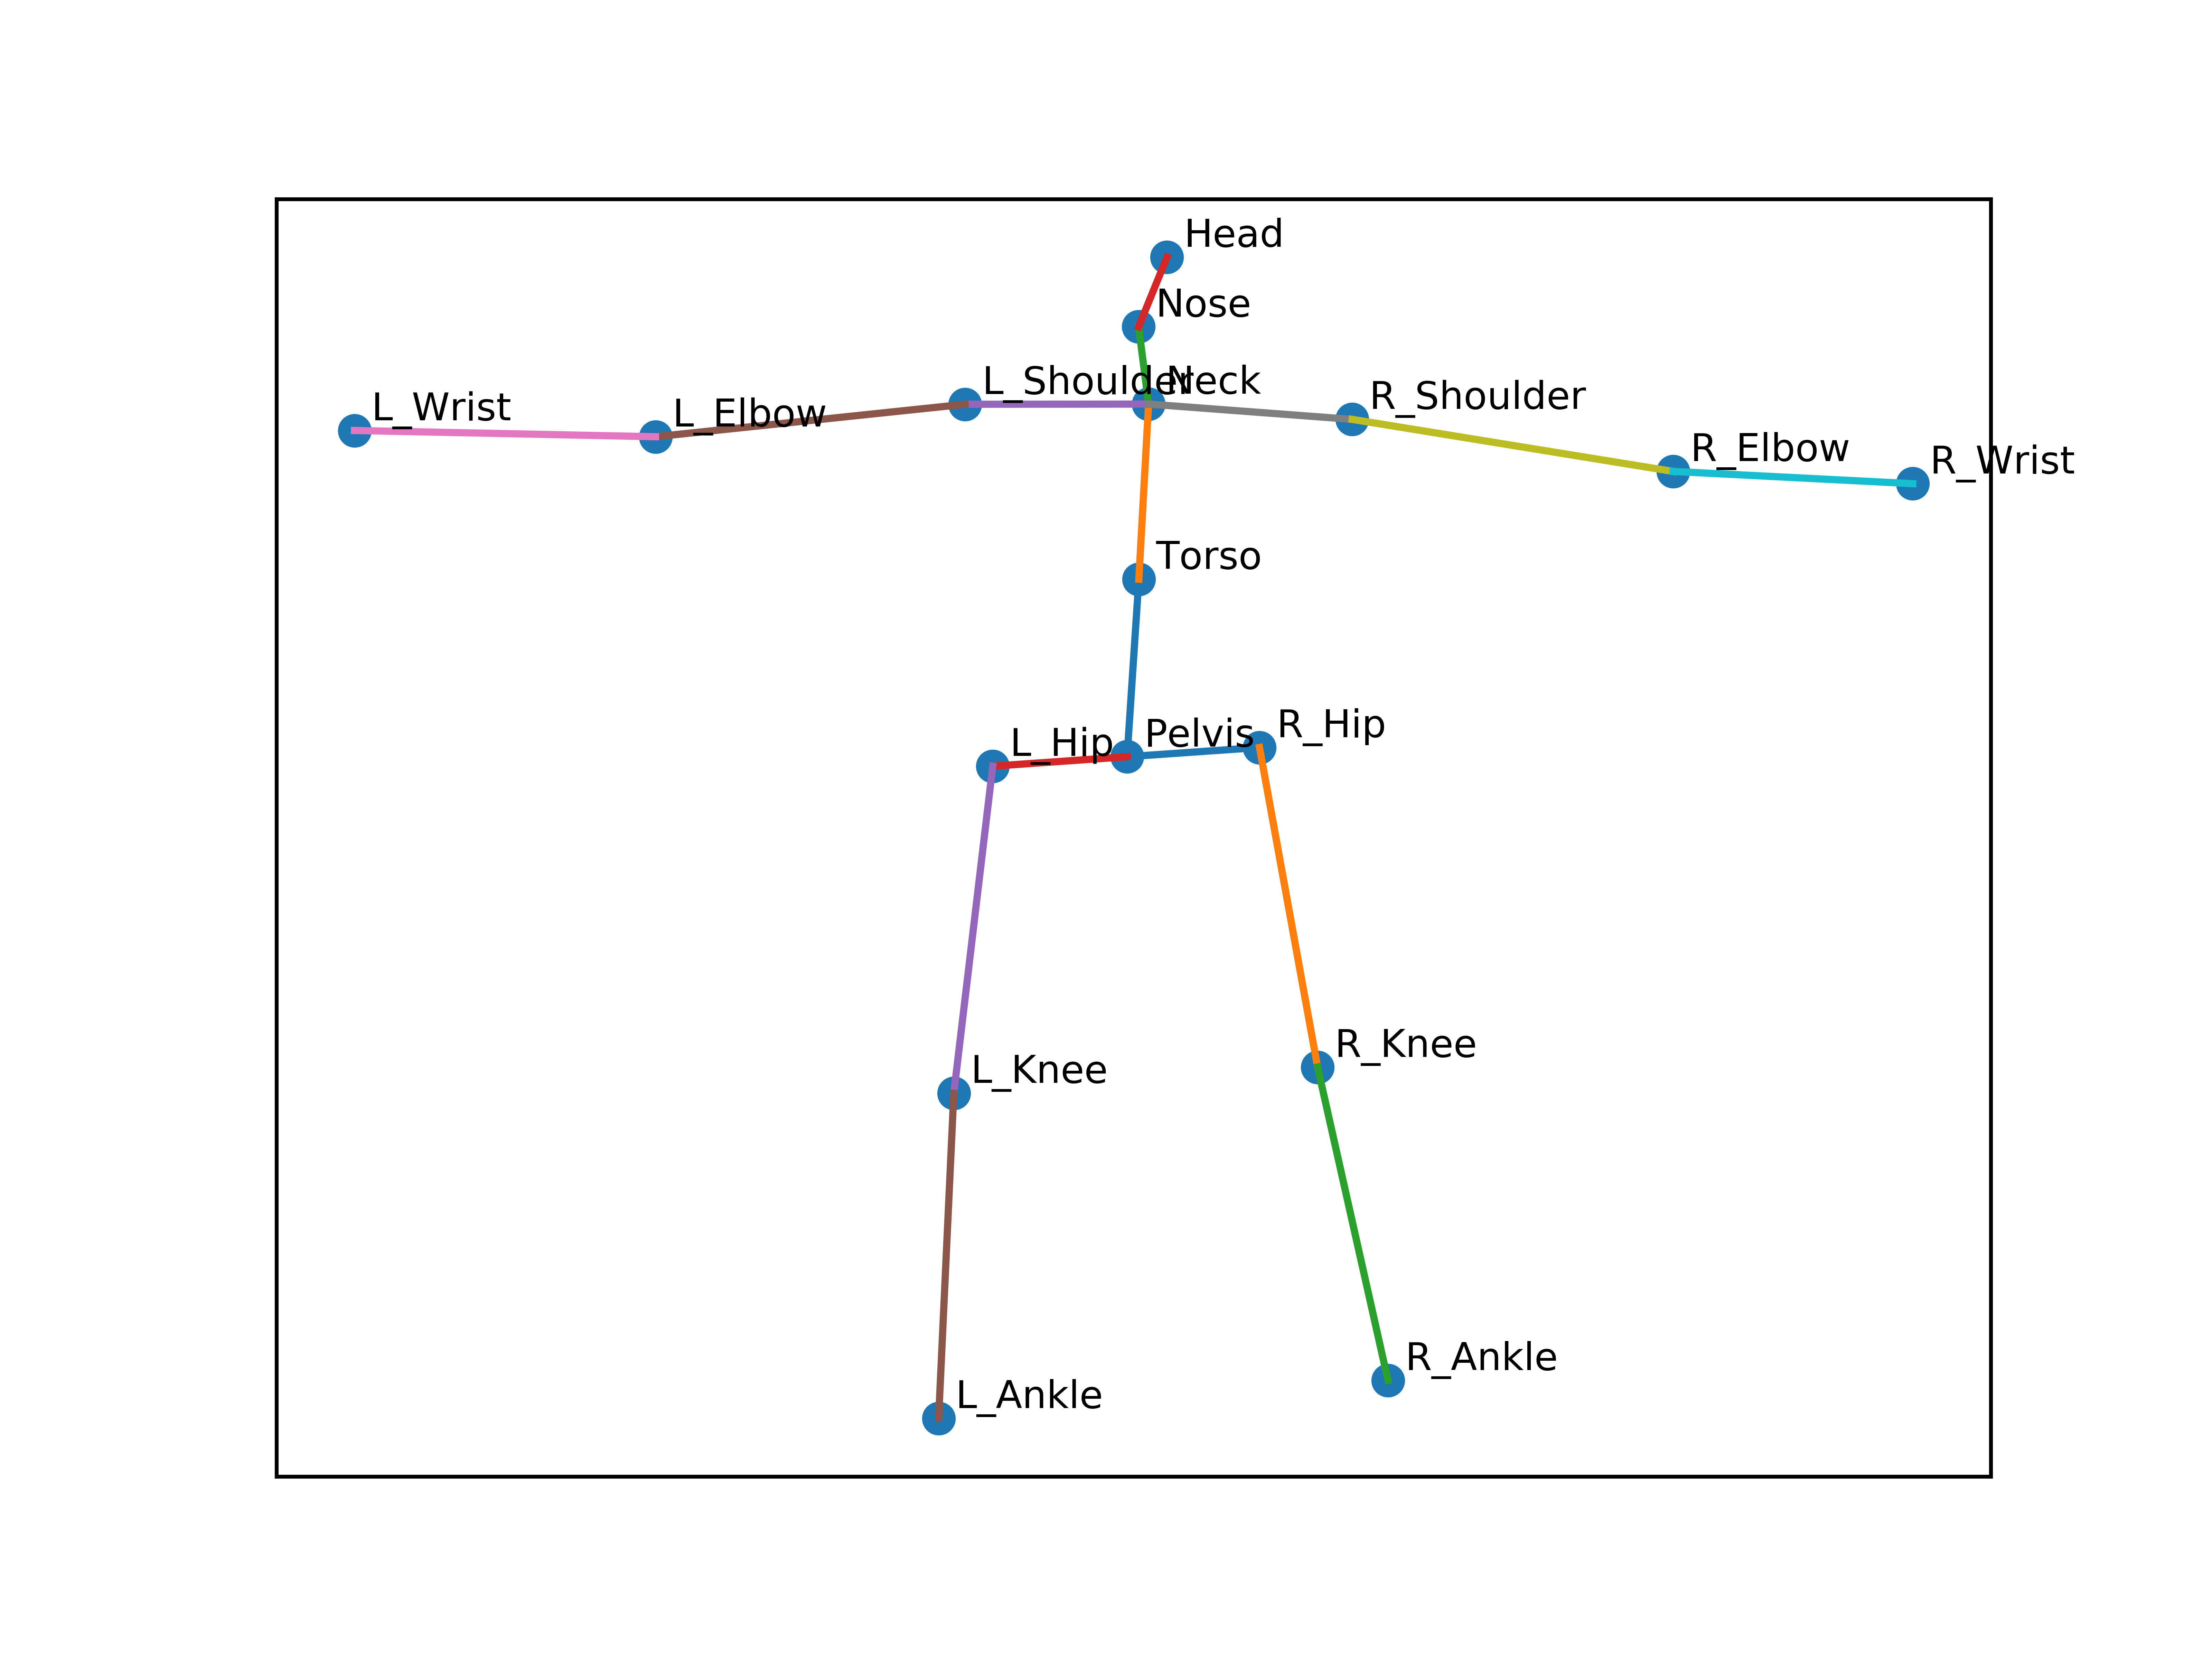
\includegraphics[width=\textwidth]{figures/h36_viz/h362d.png}
        \caption{}
    \end{subfigure}
    \hfill
    \begin{subfigure}[b]{0.3\textwidth}
        \centering
        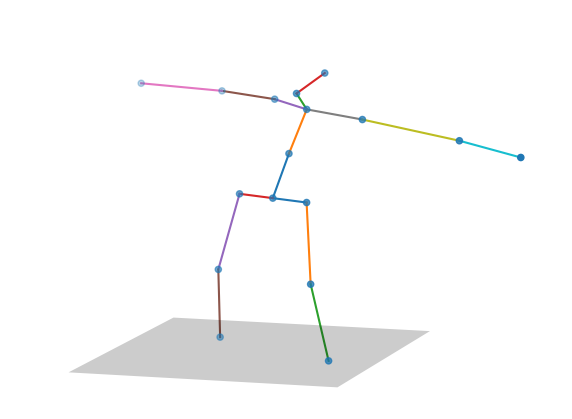
\includegraphics[width=\textwidth]{figures/h36_viz/h363d.png}
        \caption{}
    \end{subfigure}

    \caption{(a) RGB image from one of the 4 cameras. (b) Corresponding 2D pose obtained from the 3D pose to the right with joint labels. (c) Corresponding 3D pose, rotated for a better view of the spatial distribution of the joints}

    \label{fig:h36_sample}
\end{figure}

As illustrated in Fig \ref{fig:h36_data_collection}, the data is collected from a indoor environment with multiple cameras and \ac{mocap} sensors. The obtained coordinates of the 3D pose from \ac{mocap} data are global and is relative to a fixed origin the recording room. In addition to the global 3D pose, camera relative, i.e local 3D pose is also obtained using the camera's location with respect to the global origin. The global poses are useful for methods that try to exploit the multiview information and local poses that are relative to the camera can be used for absolute pose estimation. The 2D pose from each view is obtained by projection the 3D pose using the parameters of the respective camera. This 2D pose is relative to that particular camera and is with respect to the full-scale image that captures the entire scene in the camera's field of view. Along with the RGB images, global and local 3D pose and 2D pose, other metadata is available. This metadata includes intrinsic and extrinsic parameters of each camera, an identifier for each of the samples of a particular action sequence, bounding box coordinates of the human in the full-scale image, subject, action, subaction and camera ids for each sample. 

\begin{figure}[h]
    \centering
    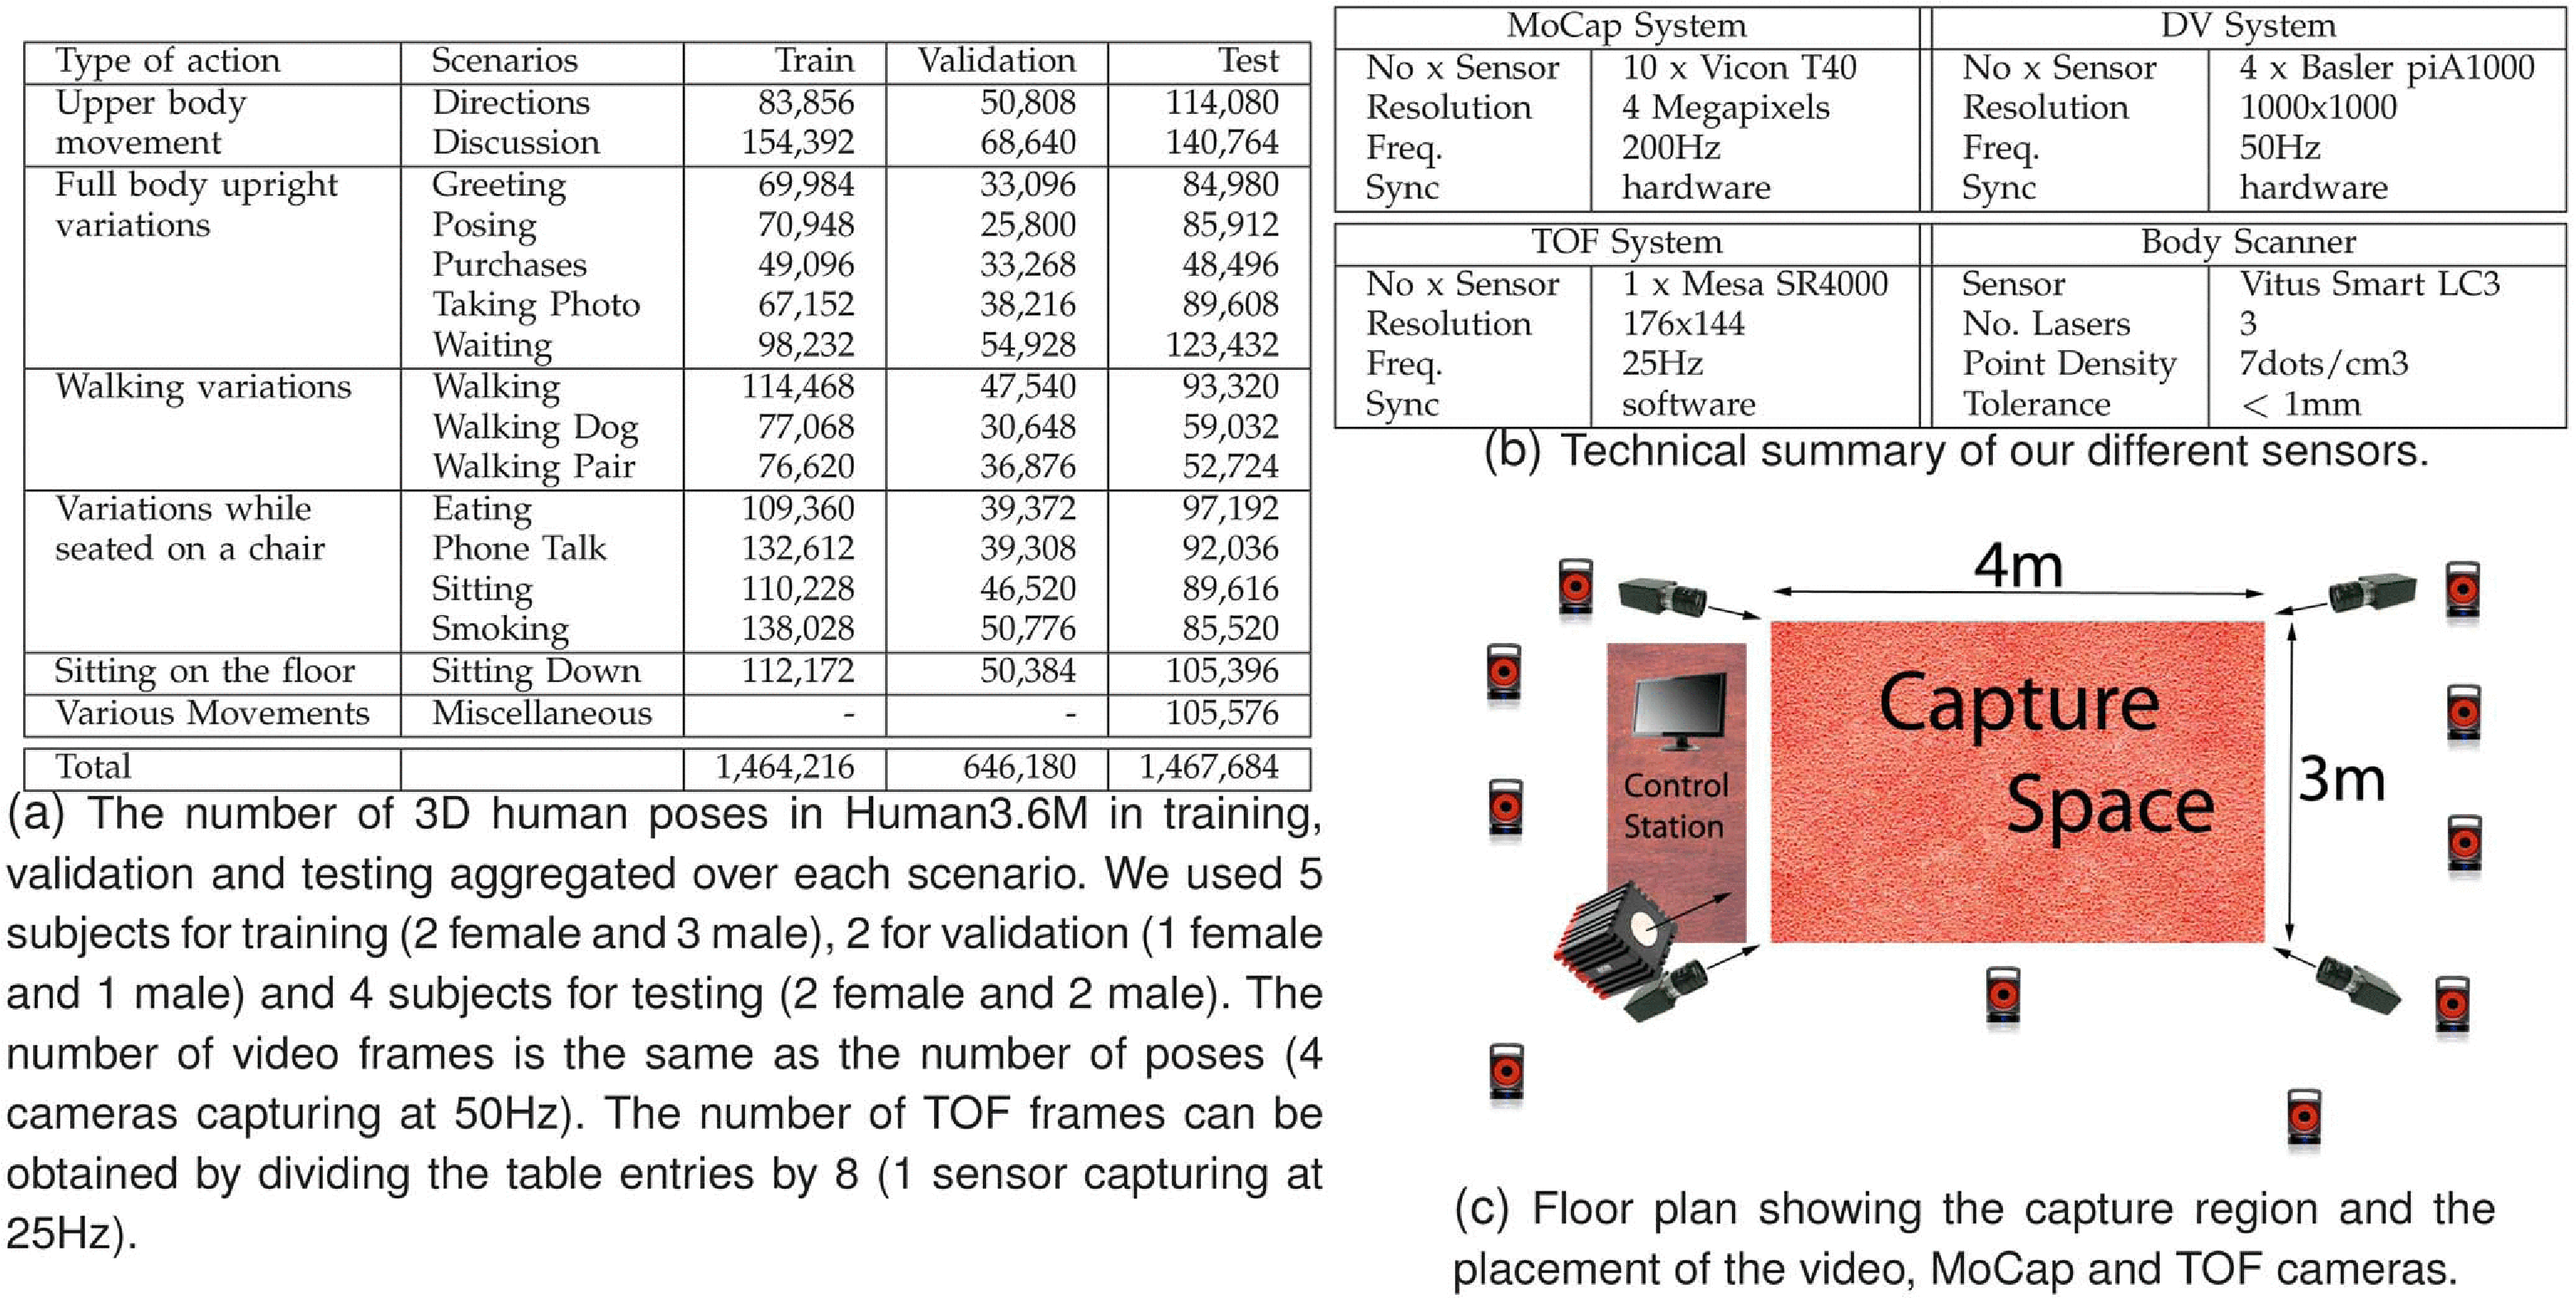
\includegraphics[width=\textwidth]{figures/h36/data_collection.pdf}
    \caption{Human3.6M data collection details. Image source \cite{H3.6}}
    \label{fig:h36_data_collection}
\end{figure}

% TODO -- Add things related to 3D projection, depth ambiguity, rigid body alignment
\section{Projective Geometry}

The projection of the poses in the thesis is using a simple pinhole camera model as illustrated in fig.\ref{fig:pinhole}. A unit camera model is assumed for the dataset and the poses are predicted around the origin and translated to a fixed image plane. Thus the error in projection is not significant. 

\begin{figure}[h]
    \centering
    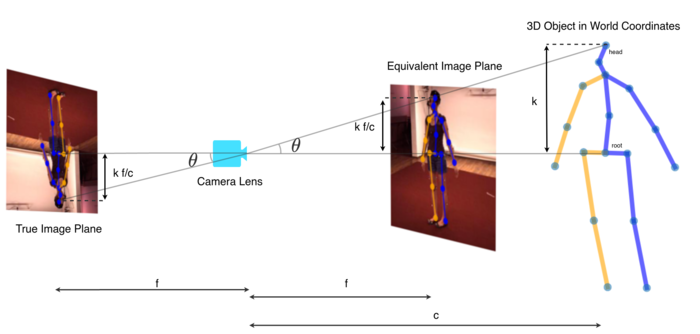
\includegraphics[scale=0.2]{figures/background/pinhole.png}
    \caption{Pinhole Camera Model. Image Source \cite{pinhole}}
    \label{fig:pinhole}
\end{figure}




% \subsection{Camera projection}
\section{Depth Ambiguity and Camera Modeling}
\label{depth_ambiguity_camera_modeling}

One of the main problems discussed in \ref{section:Related Work} is depth ambiguity. The fig \ref{fig:depthambi} illustrates the challenges in lifting 2D pose to 3D pose. During evaluation under protocol 2, the 3D poses are transformed using rigid or Procrustes alignment with the ground truth pose as illustrated in fig. \ref{fig:procrustes}. But in the proposed method we only translated and rotate but do not scale the pose.



% prtocol 2 or both protocols + scaling explanation


\begin{figure}[h]
    \centering
    \begin{subfigure}[b]{0.6\textwidth}
        \centering
        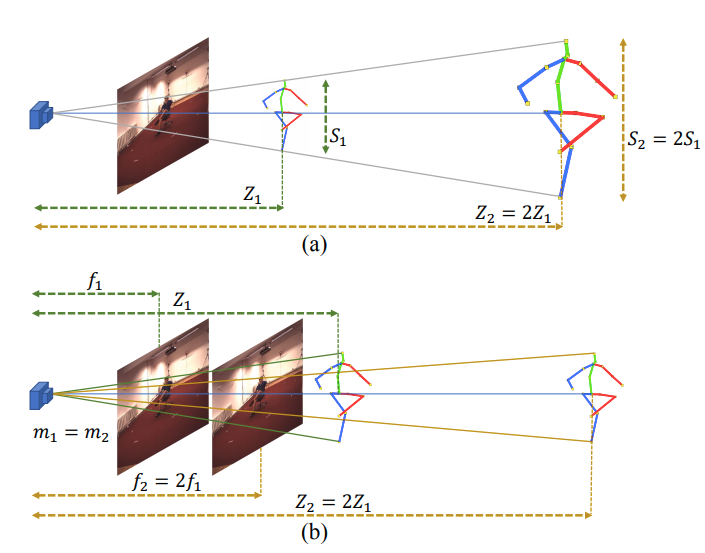
\includegraphics[width=\textwidth]{figures/background/depthambi.png}
        
    \end{subfigure}

    \begin{subfigure}[b]{\textwidth}
        \centering
        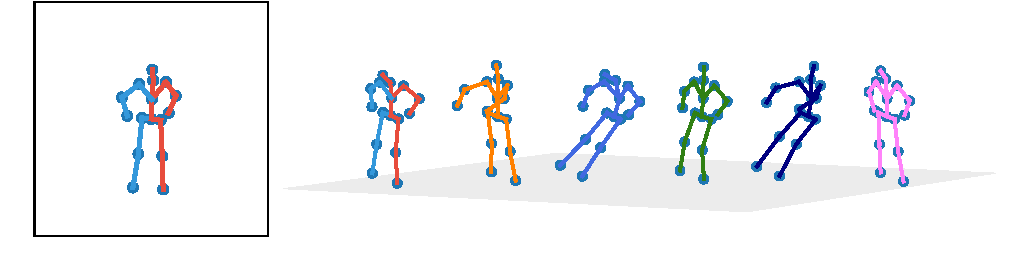
\includegraphics[width=\textwidth]{figures/h36_viz/multiple3d_per_2d.pdf}

    \end{subfigure}

    \caption{shows 2 of the infinite possible poses that result in the same 2D reprojection. Where (b) shows the same phenomenon for different focal legths
    Image Source \cite{poselifter}}
    \label{fig:depth_ambiguity_cases}
\end{figure}



%FIXME explain properly
%FIXME fix citation of pinhole



% % \lipsum[1] %FIXME
% \subsection{Depth Ambiguity and Camera Modeling}


% % \lipsum[1] %FIXME
% \subsection{Procrustes Alignment}
% % \lipsum[1-4] %FIXME


\section{Processing}

The methods explored by this thesis would require only images, 2D, and 3D human pose from the dataset. The following are the pre-processing steps for the 2D and 3D poses.


% \begin{figure}[h]
%     \centering
%     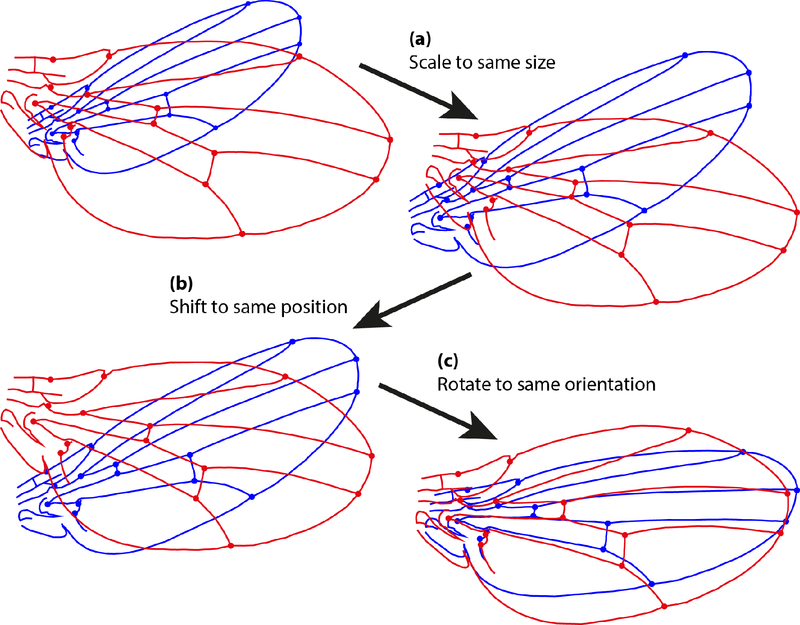
\includegraphics[scale=0.8]{figures/background/Procrustes_superimposition.png}
%     \caption{Illustration of Procrustes Alignment. Image Source \cite{Procrustes}}
%     \label{fig:procrustes}
% \end{figure}

\begin{figure}
    \centering
    \begin{subfigure}[b]{0.25\textwidth}
        \centering
        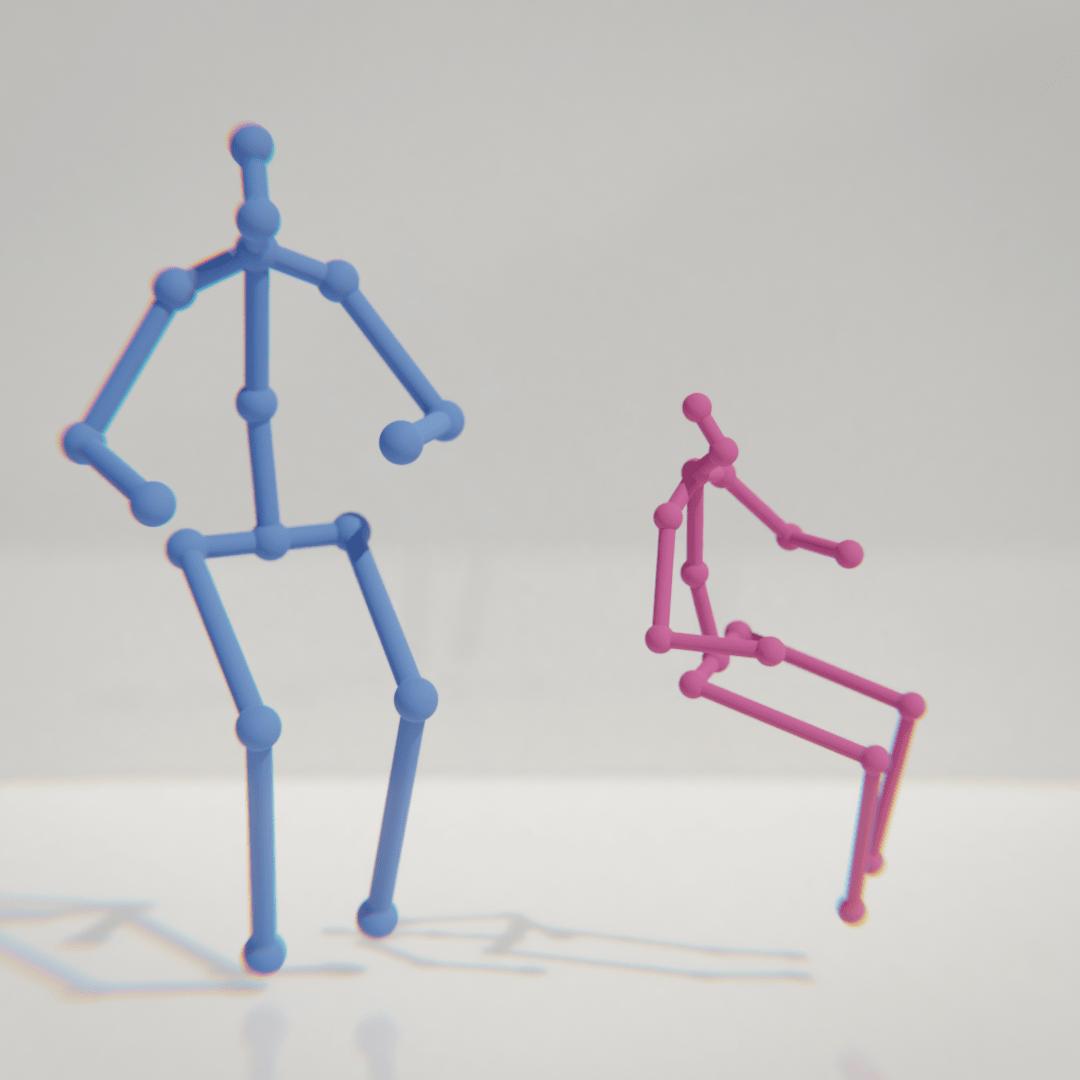
\includegraphics[width=\textwidth]{figures/h36_viz/proc_raw.png}
        \caption{$y=x$}
        \label{fig:y equals x}
    \end{subfigure}
    \hfill
    \begin{subfigure}[b]{0.25\textwidth}
        \centering
        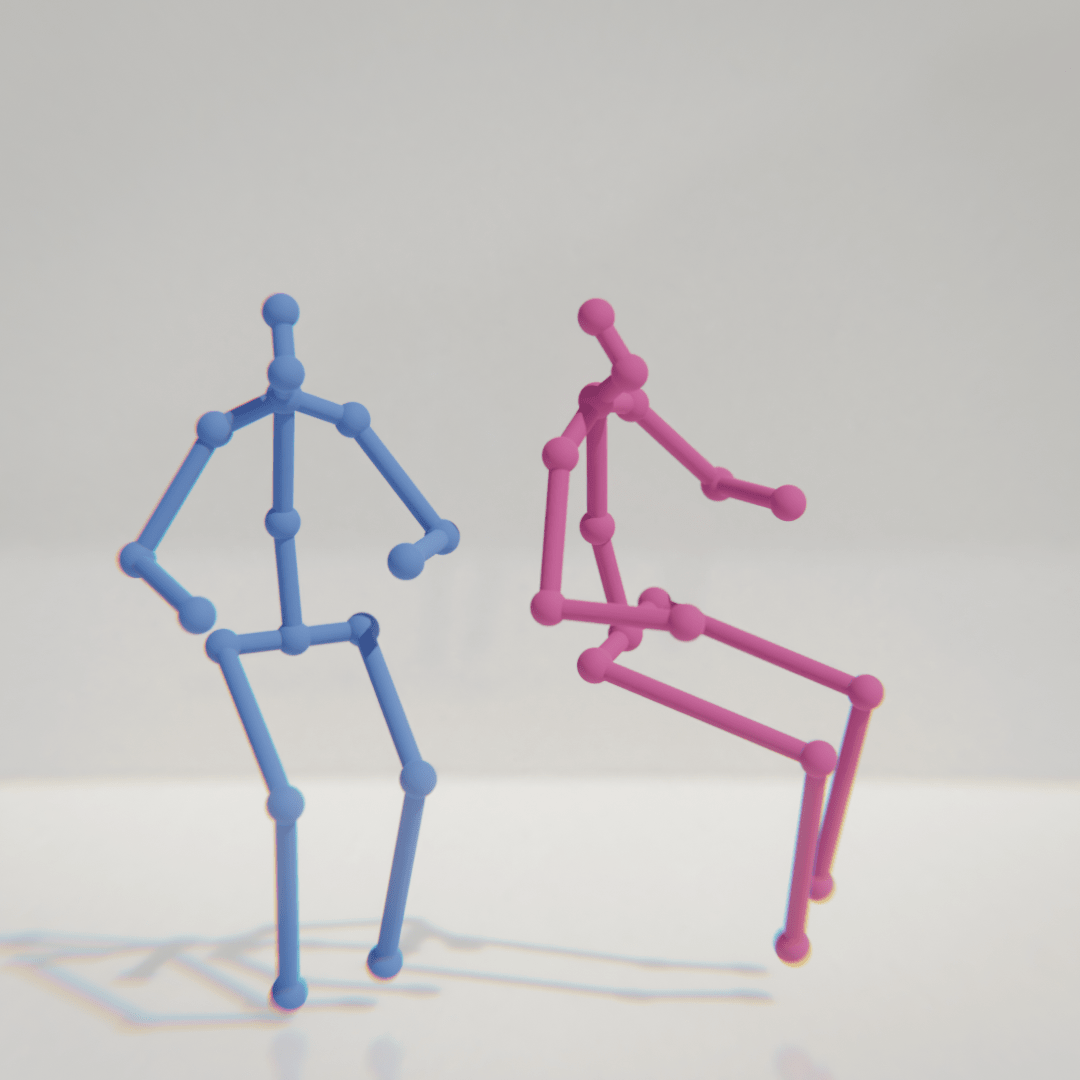
\includegraphics[width=\textwidth]{figures/h36_viz/proc_scale.png}
        \caption{$y=3sinx$}
        \label{fig:three sin x}
    \end{subfigure}
    \hfill
    \begin{subfigure}[b]{0.25\textwidth}
        \centering
        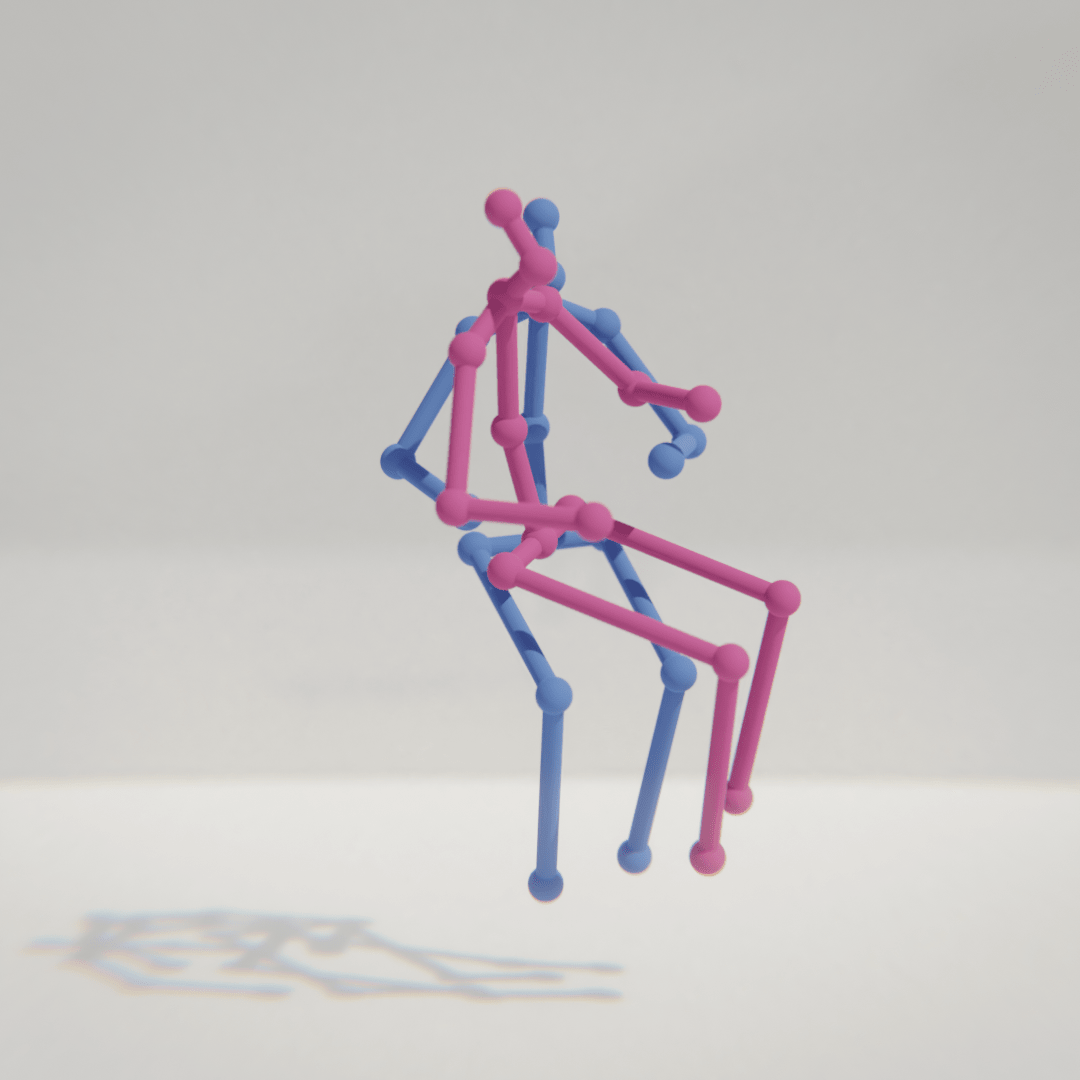
\includegraphics[width=\textwidth]{figures/h36_viz/proc_pos.png}
        \caption{$y=5/x$}
        \label{fig:five over x}
    \end{subfigure}
    \hfill
    \begin{subfigure}[b]{0.25\textwidth}
        \centering
        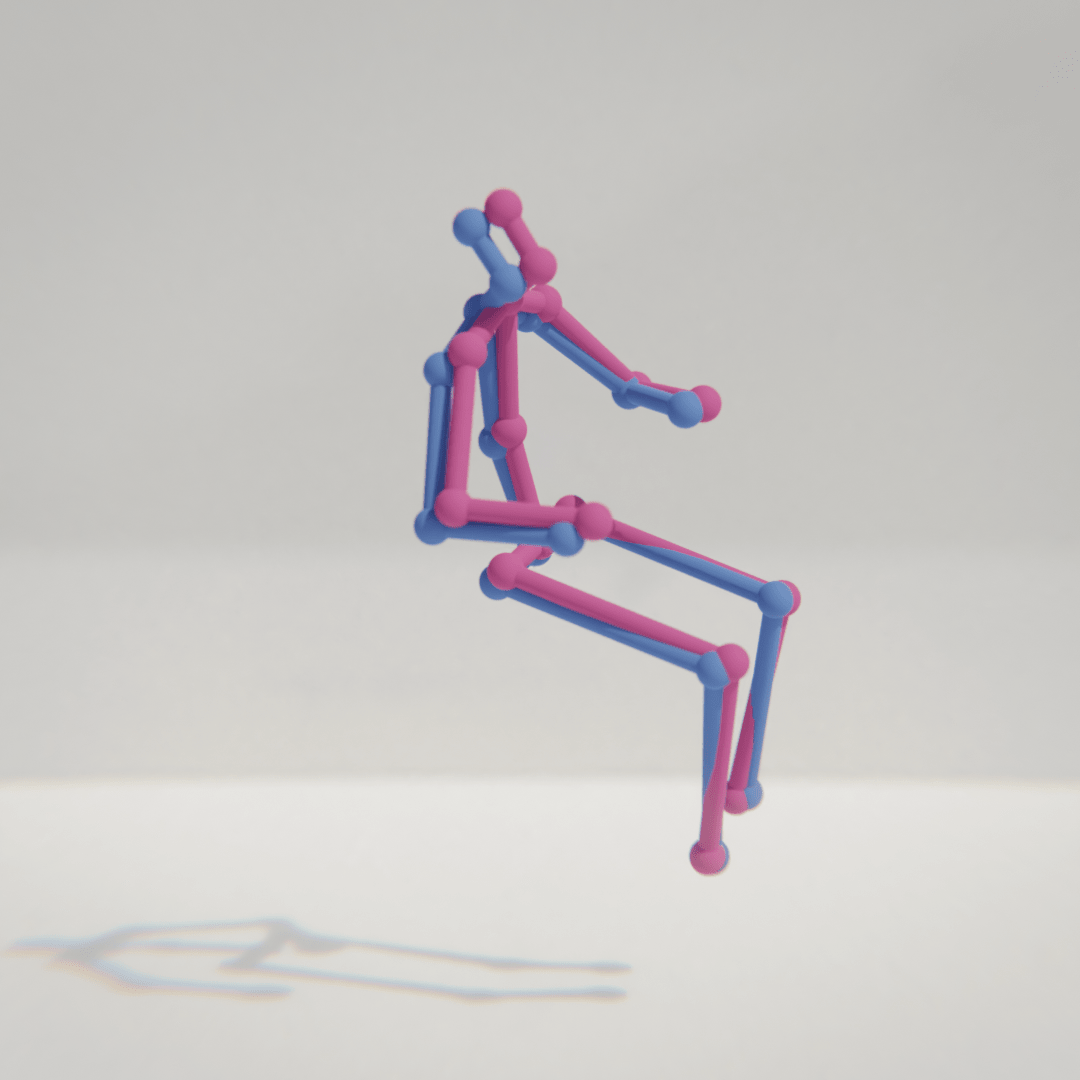
\includegraphics[width=\textwidth]{figures/h36_viz/proc_rot.png}
        \caption{$y=5/x$}
        \label{fig:five over x}
    \end{subfigure}
    \caption{Three simple graphs}
    \label{fig:procrustes}
\end{figure}

The 3D pose in the dataset that is obtained from the marker-based \ac{mocap} is in a global reference frame. These poses using the camera parameters are transformed into the camera coordinate frame. For the task of predicting 3D pose from either images or 2D pose, it is unrealistic to directly estimate all the joints of the pose in a global frame. So the first step of processing would be to zero the pose w.r.t the root joint say, Pelvis. As the root is always zero, we remove it so we do not have to learn the constant joint. Removing Pelvis, 16 out of the 17 joints or keypoints remain. The 3D pose is further scaled in down so that the distance between the root and the head is 1. This results in numerical stability during training.


The 2D pose which is obtained from the 3D pose, is also in the camera coordinate frame. The 2D pose is also zeroed and scaled so that the distance between the root and head is 1/c units. Where c is a constant distance at which the image plane is fixed. As a unit camera or camera with unit focal length is assumed the projection of unit 3D poses onto a plane at a fixed distance of 1/c units. The root of the 2D pose is however removed to remain consistent with the 3D pose.

% TODO update - experiments are yet to be done
% TODO link MPJPE to its explanation in other chapter or sections

The estimated poses from the networks that are trained on downscaled poses are upscaled to the original size using for valuation. This postprocessing step is required for getting the distance between prediction and ground truth keypoints in true units of millimeters.

